\documentclass[11pt, a5paper, parskip=half-, DIV=12]{scrartcl}

\usepackage{../endeavour}
\usepackage{../endeavour_book}

% Hack to allow relative path here
\tikzset{starfield/.pic={
	\node () at (current page.center) {
\includegraphics[width=\pagewidth, height=\pageheight]{../Images/starfield.png}};
}}

\version{0.1}

\begin{document}
% Colour Cover
\thispagestyle{plain}
\AddToShipoutPictureBG{
\begin{tikzpicture}[remember picture, overlay]
	\node () at (current page.center) {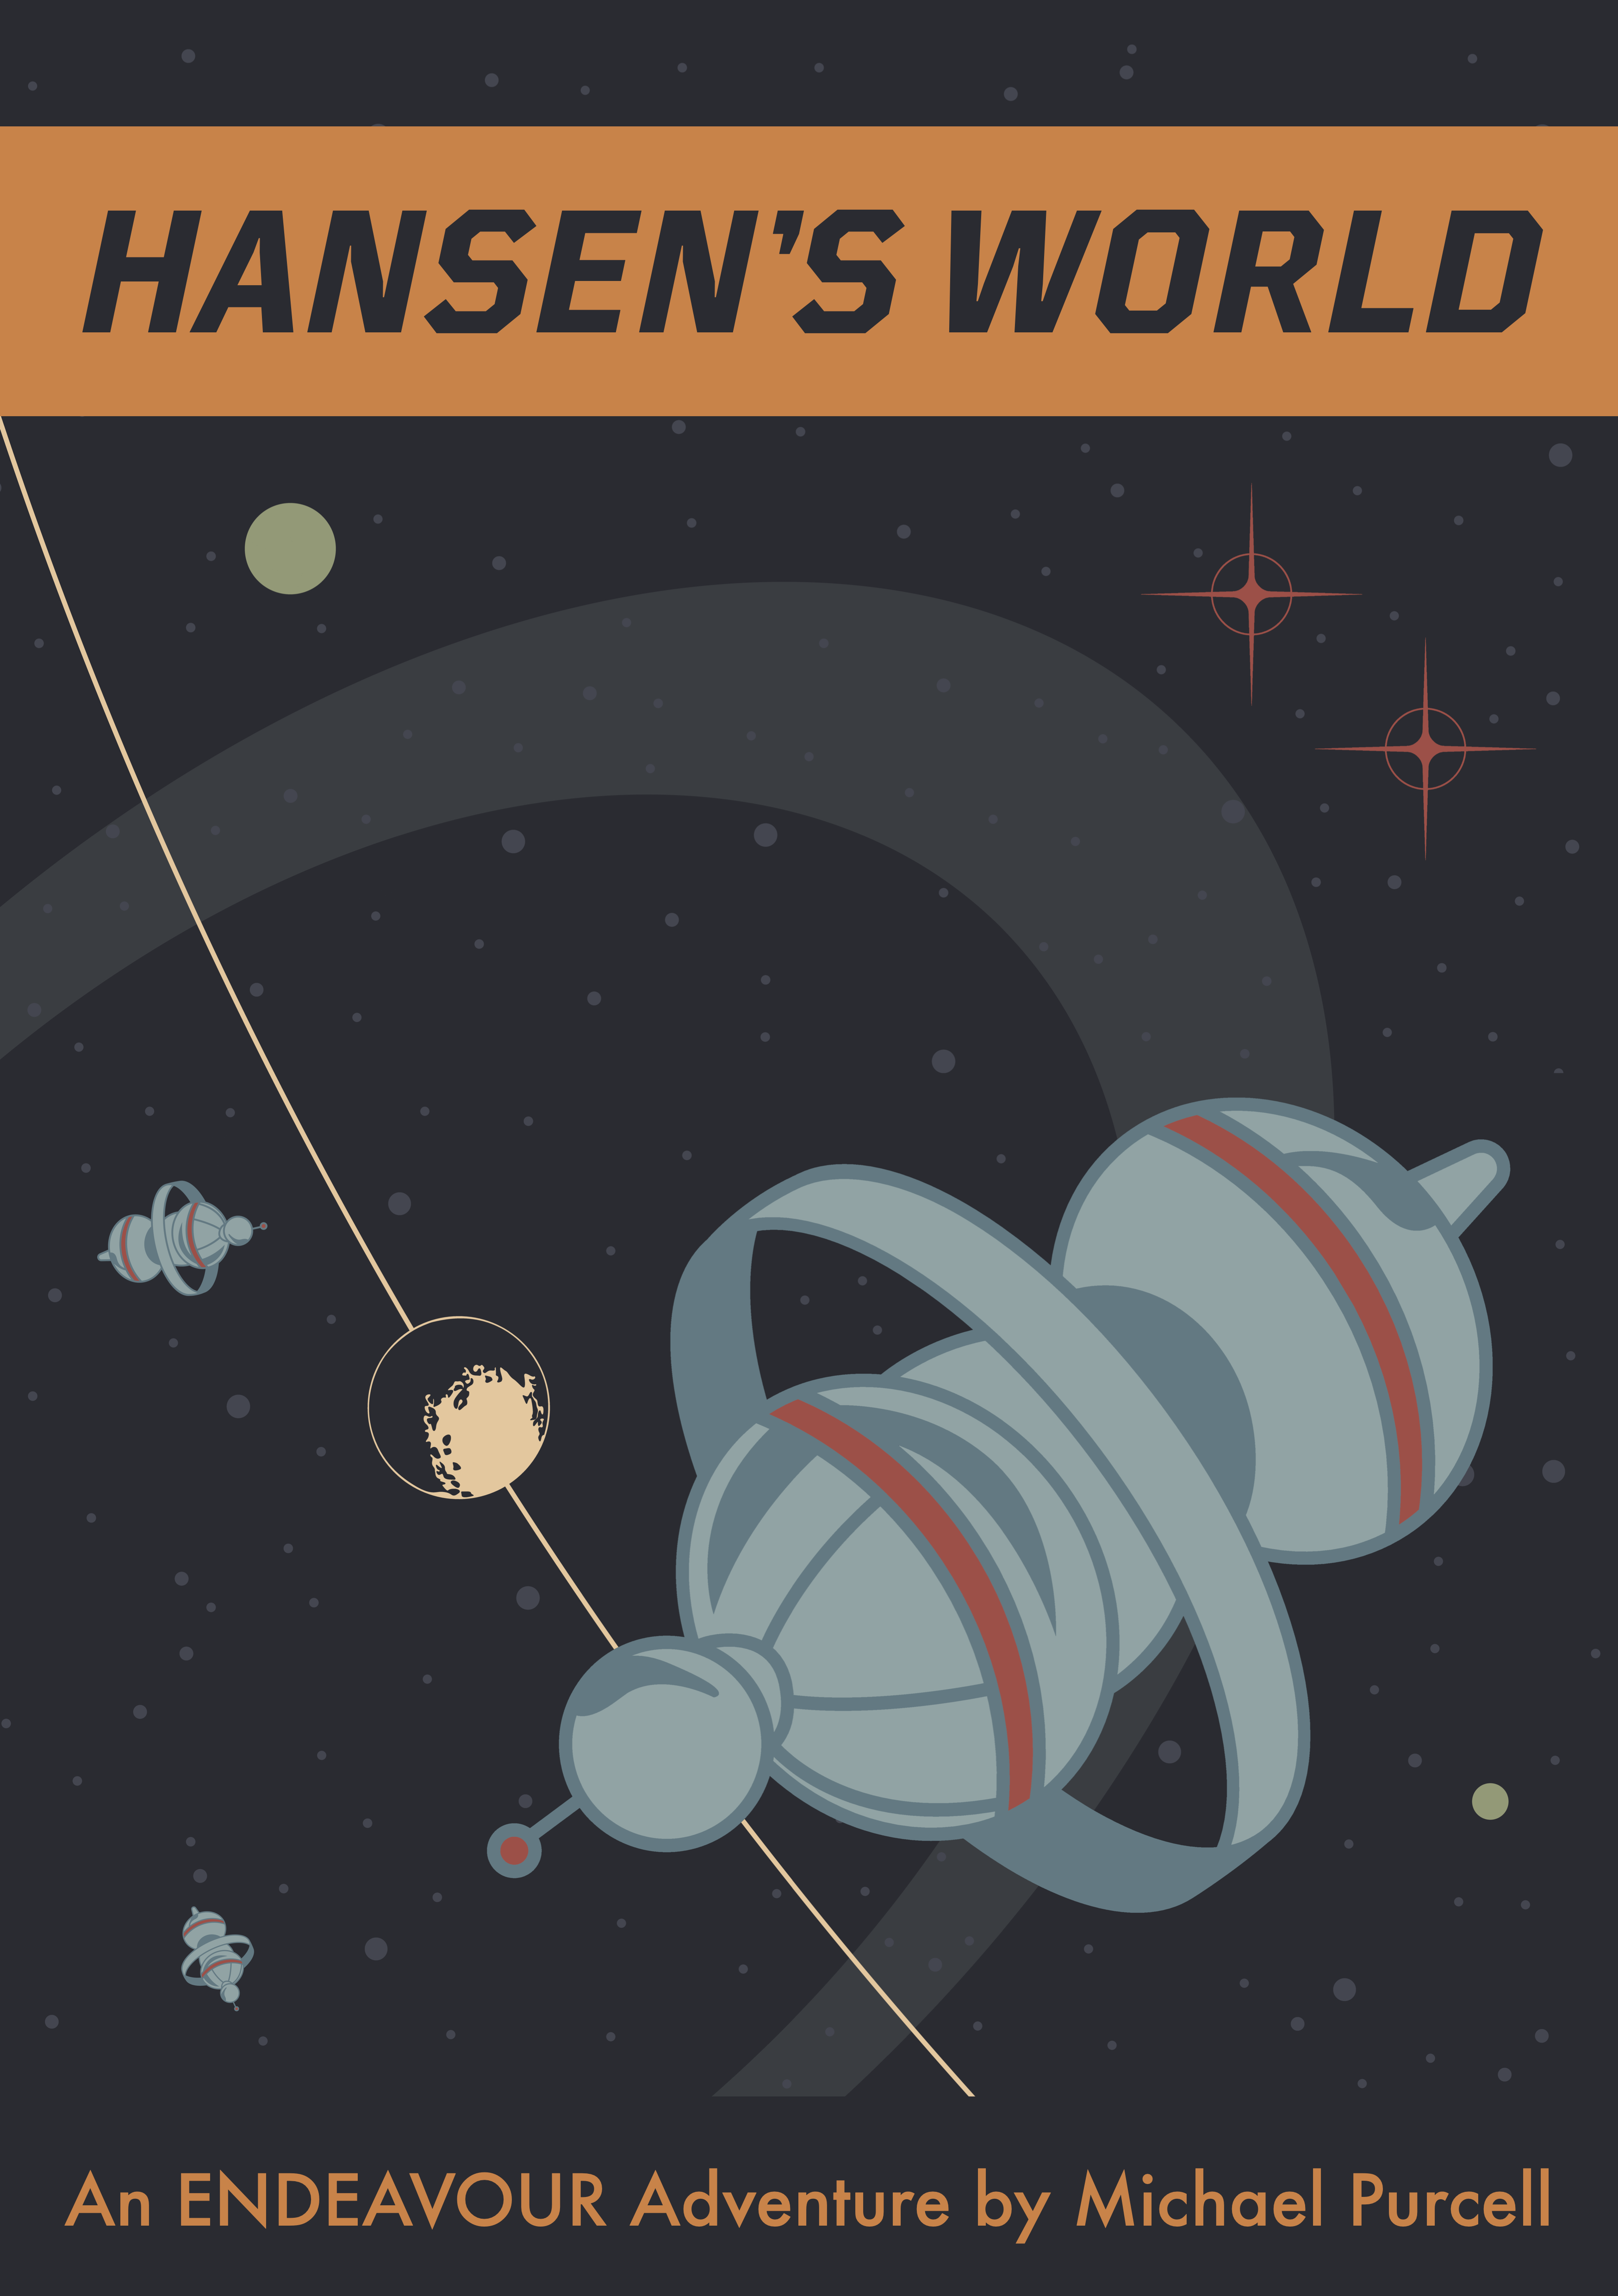
\includegraphics[width=\pagewidth, height=\pageheight]{../Images/hansens_world_cover.png}};
\end{tikzpicture}
}
{
\colorlet{headfootcolor}{LCARS_ORANGE}
\phantom{a}

\newpage
}

\ClearShipoutPicture
\AddToShipoutPictureBG{
	\begin{tikzpicture}[remember picture, overlay]
	\pic () at (current page.center) {starfield};
		\node[endeavour_box, minimum width=12.6cm, minimum height=18.8 cm] at (current page.center) {};
	\end{tikzpicture}
}

\setcounter{page}{1}
\setmainfont{TeX Gyre Schola}
\normalsize
\raggedright

\section*{Planet Name}
\textit{\textbf{Captain's Log:} Introduce the planet and any required exposition.}

\subsection*{Arrival}
A first challenge for the players to face.  This challenge should introduce the major theme of the adventure.

\subsubsection*{Challenge Name}
\begin{itemize}
	\item \textit{Will you \dots?} \textbf{Domain} vs. \textbf{Opponent}. \\ Additional details.
	\item \textit{Or will you \ldots?} \textbf{Domain} vs. \textbf{Opponent}. \\ Additional details.  
\end{itemize}

\newpage

\subsection*{Trials}
\subsubsection*{First Trial}
A situation that advances the story. \textit{Ask a leading question that suggests a possible challenge.} \textbf{Domain} vs. \textbf{Opponent}.

\subsubsection*{Second Trial}
A situation that advances the story. \textit{Ask a leading question that suggests a possible challenge.} \textbf{Domain} vs. \textbf{Opponent}.

\subsubsection*{Third Trial}
A situation that advances the story. \textit{Ask a leading question that suggests a possible challenge.} \textbf{Domain} vs. \textbf{Opponent}.

\subsection*{Crisis}

\begin{itemize}
	\item \textit{Will you \ldots?} \textbf{Threats:} Two or three threats.
	\item \textit{Or will you \ldots?} \textbf{Threats:} Two or three threats.
\end{itemize}

\newpage

\subsection*{Characters}
\begin{description}
	\item[Character Name (d?):] Epithet (d?), \ldots
	\item[Character Name (d?):] Epithet (d?), \ldots
	\item[Character Name (d?):] Epithet (d?), \ldots
\end{description}

\subsection*{Places}
\begin{description}
	\item[Place Name:] Brief description.
	\item[Place Name:] Brief description.
	\item[Place Name:] Brief description.
\end{description}

\subsection*{Mysteries}
\begin{description}
	\item[A fact about the planet.] \phantom{a} \\ A few related facts. \textit{One or two related questions.}
	\item[A fact about the planet.] \phantom{a} \\ A few related facts. \textit{One or two related questions.}
\end{description}
\end{document}